\documentclass{beamer}
\usepackage{polski}
\usepackage{listings}
\usepackage{ulem}
\usetheme{Dresden}
%\useoutertheme[footline=authortitle,subsection=false]{miniframes}
%\usecolortheme{dolphin}

\author{Piotr Rogula}
\title{Analiza statystyczna czasów na wykonywanie ruchów w
	szachach}
\institute[Pwr]{Politechnika Wrocławska}
\begin{document}
	\bibliographystyle{plain}
\begin{frame}[plain]
    \maketitle
    \begin{center}
    	pod promotorstwem prof. dr hab. inż. Marcina Magdziarza
    \end{center}
\end{frame}

\section{Wstęp}

\begin{frame}{Spis treści}

\begin{enumerate}
\item wstęp
	\begin{enumerate}
		\item motywacja
		\item kluczowe wyniki innych autorów
		\item potrzebne oznaczenia
	\end{enumerate}
\item wyniki własne
	\begin{enumerate}
		\item sformułowanie problemu
		\item dane
		\item analiza problemu
	\end{enumerate}
\item podsumowanie
\end{enumerate}

\end{frame}

%\begin{frame}{Motywacja}
%\begin{enumerate}
%	\item Szachy jako hobby
%\end{enumerate}	
%\end{frame}
%	\begin{frame}{Motywacja}
%		\begin{enumerate}
%			\item Szachy jako hobby
%			\item popularny temat
%		\end{enumerate}	
%	\end{frame}
		\begin{frame}{Motywacja}
			\begin{enumerate}
				\item Szachy jako hobby
				\item popularny temat
				\item niedosyt literatury opisującej dane zagadnienie
			\end{enumerate}	
		\end{frame}


%%% Kluczowe wyniki innych autorów
\begin{frame}{Kluczowe wyniki innych autorów}
	\begin{itemize}
		\item System Elo \cite{elo} (Arpad Elo)
	\end{itemize}
\end{frame}

\begin{frame}{System Elo}
	\begin{itemize}
		\item przyznawanie punktów bazujące na różnicy rankingu graczy
		\item pierwszy system mający podłoże probabilistyczne
	\end{itemize}
\end{frame}

\begin{frame}{Kluczowe wyniki innych autorów}
	\begin{itemize}
		\item System Elo \cite{elo} (Arpad Elo)
		\item System Glicko-2 \cite{glicko}  (Mark Glickman)
	\end{itemize}
\end{frame}

\begin{frame}{System Glicko-2}
	\begin{itemize}
		\item ulepszenie systemu Elo.
		\begin{itemize}
			\item wzięcie pod uwagę przedziału ufności rankingu każdego z graczy.
		\end{itemize}
		\item używany w dużej liczbie gier MMO.
	\end{itemize}
\end{frame}

\begin{frame}{Kluczowe wyniki innych autorów}
	\begin{itemize}
		\item System Elo \cite{elo} (Arpad Elo)
		\item System Glicko-2 \cite{glicko} (Mark Glickman)
		\item Silnik Stockfish \cite{stockfish}
	\end{itemize}
\end{frame}



\begin{frame}{Silnik Stockfish}
	\begin{itemize}
		\item funkcja oceny
	\end{itemize}
	wynik liniowej funkcji 
	ważonej sumy cech, na którą składają się między innymi:\\
	$f_b,f_c$ -- wartość figur odpowiednio białych i czarnych\\
	$k_b,k_c$ -- bezpieczeństwo króla odpowiednio białych i czarnych\\
	$m_b,m_c$ -- mobilność figur odpowiednio białych i czarnych\\
	$z_b,z_c$ -- potencjalne zagrożenia wykonane odpowiednio białych i czarnych\\
	\begin{equation*}
		f(f_b,f_c,k_b,k_c,m_b,m_c,\dots)=c_1(f_b-f_c)+c_2(k_b-k_c)+c_3(m_b-m_c)+\dots
	\end{equation*}
	gdzie:
	$c_i$ są stałymi określającymi wagę danej pary zmiennych.
\end{frame}

\begin{frame}{Silnik Stockfish}
	\begin{itemize}
		\item rodzaje błędów szachowych
		\begin{itemize}
			\item ??\hphantom{!} -- błąd (ang. \textit{blunder})
			\item ?\hphantom{?!}  -- pomyłka (ang. \textit{mistake}), posunięcie błędne w mniejszym stopniu niż ,,błąd''
			\item ?!\hphantom{?} -- niedokładność  (ang. \textit{innacuracy}), posunięcie, które można zastąpić zdecydowanie lepszym.
		\end{itemize}
	\end{itemize}
\end{frame}

\begin{frame}{Potrzebne oznaczenia}
	\begin{itemize}
		\item \textbf{ruch} składa się z dwóch posunięć - 1 białych i 1 czarnych
		\begin{itemize}
			\item wyjątkiem może być ostatni ruch, gdy po posunięciu białych nastąpił koniec partii.
		\end{itemize}
		\item oznaczenia posunięcia jako ,,błąd'' i ,,duży błąd'' są tożsame
		\item oznaczenie ,,pomyłka'' jest rozróżnialne od oznaczenia ,,błąd'' -- drugie jest wg silnika gorszym posunięciem
	\end{itemize}
\end{frame}


\section{Wyniki własne}

\begin{frame}{sformułowanie problemu}
	\begin{itemize}
		\item zbadanie zależności pomiędzy czasem poświęconym na wykonanie ruchu, a jego dokładnością
		\item zbadanie zależności między numerem ruchu, a czasem na jego wykonanie oraz jego dokładnością
		\item \sout{próba wyznaczenia optymalnego czasu na wykonanie ruchu\\ minimalizacja ryzyka wystąpienia błędu} 
	\end{itemize}
\end{frame}

\begin{frame}{dane}
	\begin{itemize}
		\item baza danych \textbf{Lichess.com} - 1 plik 72Gb
		\item zbadanie 2 najczęściej granych formatów (600+0, 300+0)
		\item stworzenie bazy ok. 7\% gier ocenionych przez silnik
		\item stworzenie bazy wszystkich ruchów ze wszystkich gier
		\begin{itemize}
			\item 17,52 mln posunięć z 275,94 tyś gier
		\end{itemize}
	\end{itemize}
\end{frame}

\begin{frame}{wstępna analiza}
	\begin{figure}[H]
		\centering
		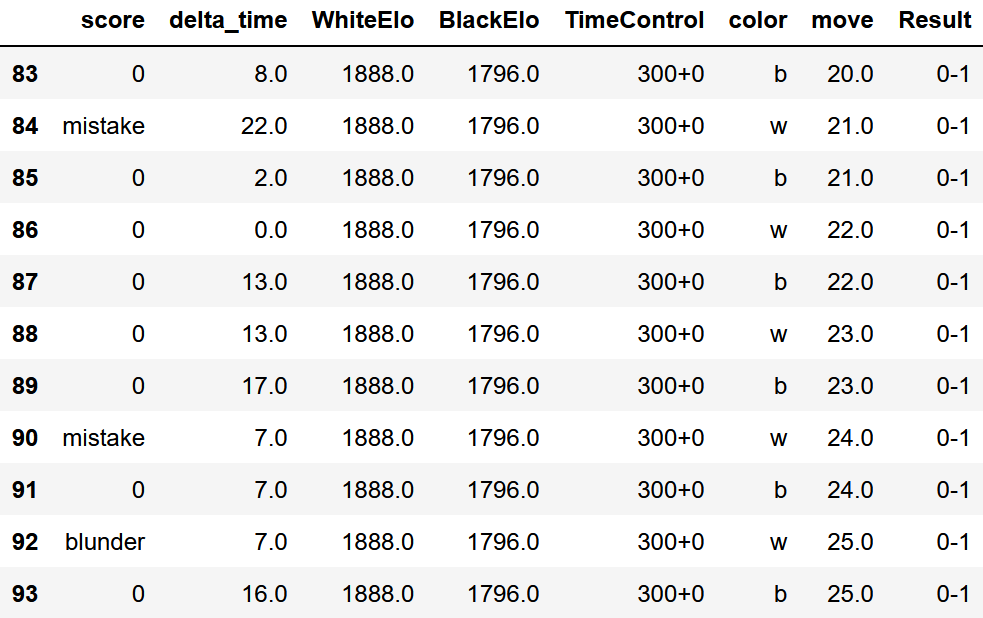
\includegraphics[width=8cm]{../Formatka/danee.png}
		\caption{Fragment bazy zawierającej ruchy z gier o formatach czasowych ,,300+0'' i ,,600+0''.}
		\label{rys:baza_ruchow}
	\end{figure}
\end{frame}

\begin{frame}{dane}
		\begin{itemize}
	\item czego nie ma w danych?
		\begin{itemize}
		\item digitalizacja czasu -- czas na posunięcie zaokrąglony do pełnych sekund
		\item brak informacji i odpowiedniej miary dotyczącej skomplikowania sytuacji na szachownicy
	\end{itemize}
	\end{itemize}
\end{frame}



\begin{frame}{Analiza problemu - wstępny przegląd danych}

	\begin{figure}[H]
		\centering
		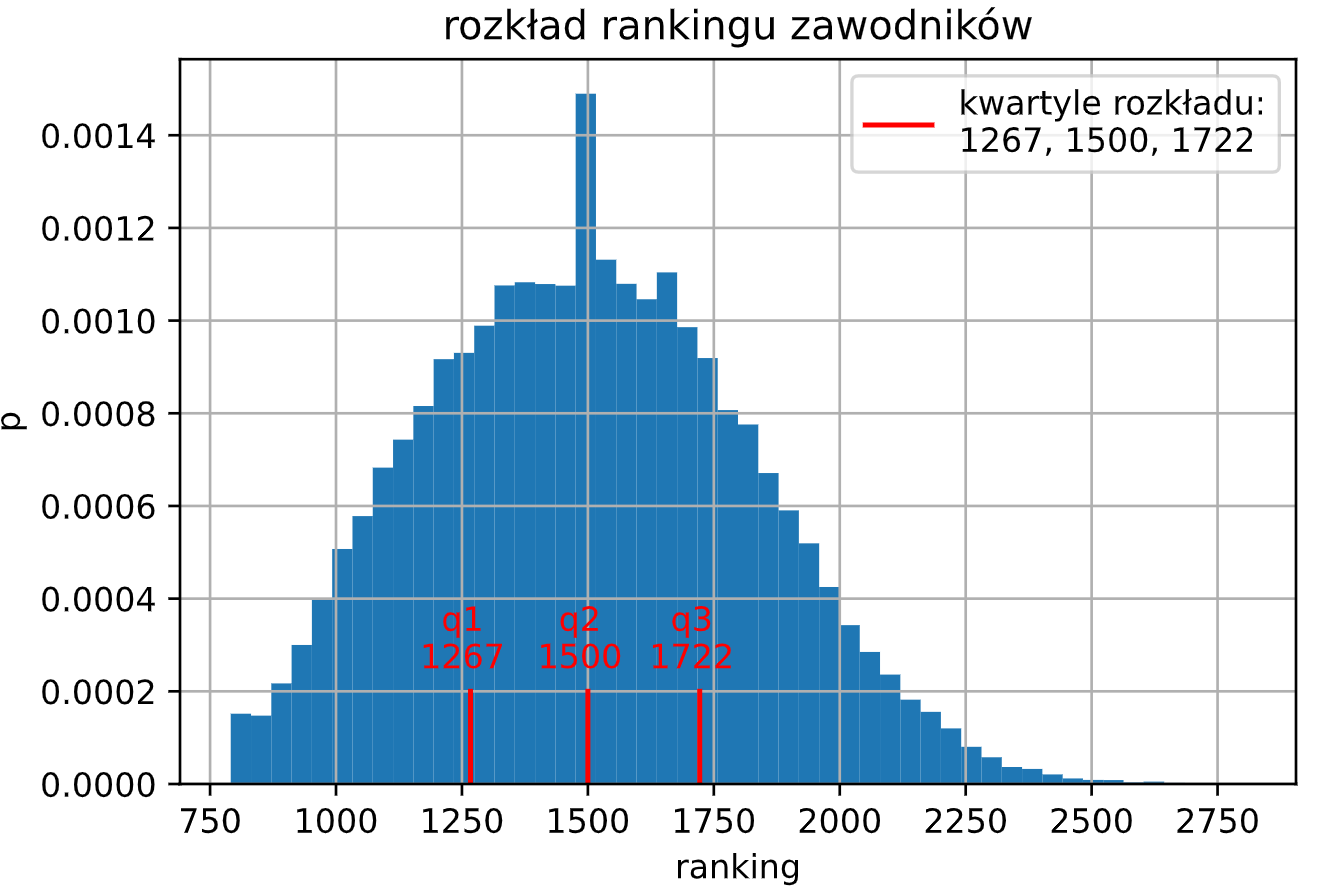
\includegraphics[width=8cm]{../Formatka/ranking.png}
		\caption{rozkład rankingu zawodników wraz z zaznaczonymi kwartylami}
		\label{rys:rozklad_elo}
	\end{figure}
\end{frame}

\begin{frame}{Analiza problemu - wstępny przegląd danych}
	\begin{figure}[H]
		\centering
		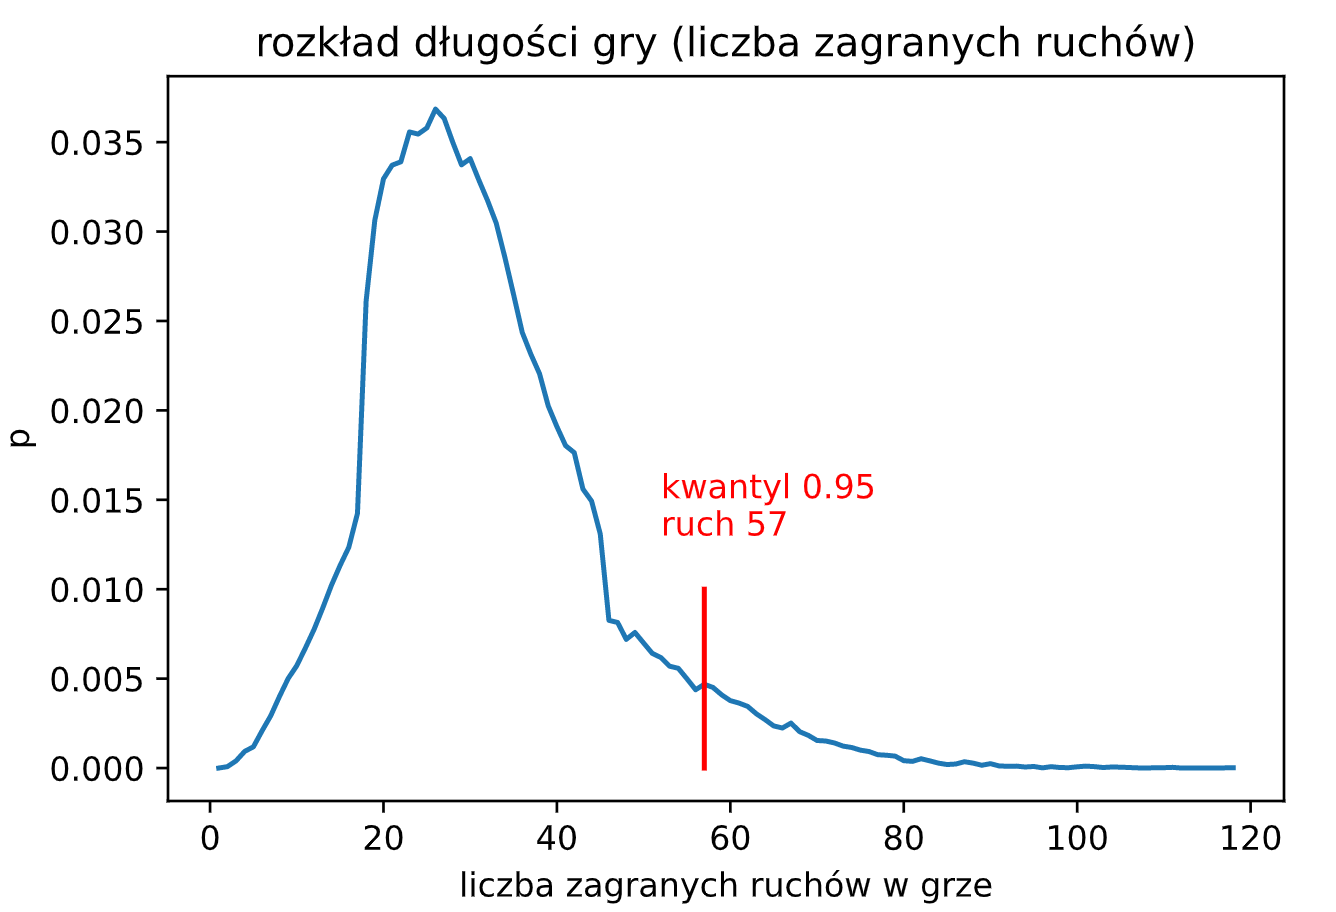
\includegraphics[width=8cm]{../Formatka/dlugosc_gry.png}
		\caption{rozkład długości gier wraz z zaznaczonym kwantylem rzędu 0.95,  dla gier z formatu 300+0 oraz 600+0.}
		\label{rys:dlugosc_gier}
	\end{figure}
\end{frame}

\begin{frame}{Zależność między indeksem ruchu, a poświęconym czasem}
	\begin{figure}[H]
		\centering
		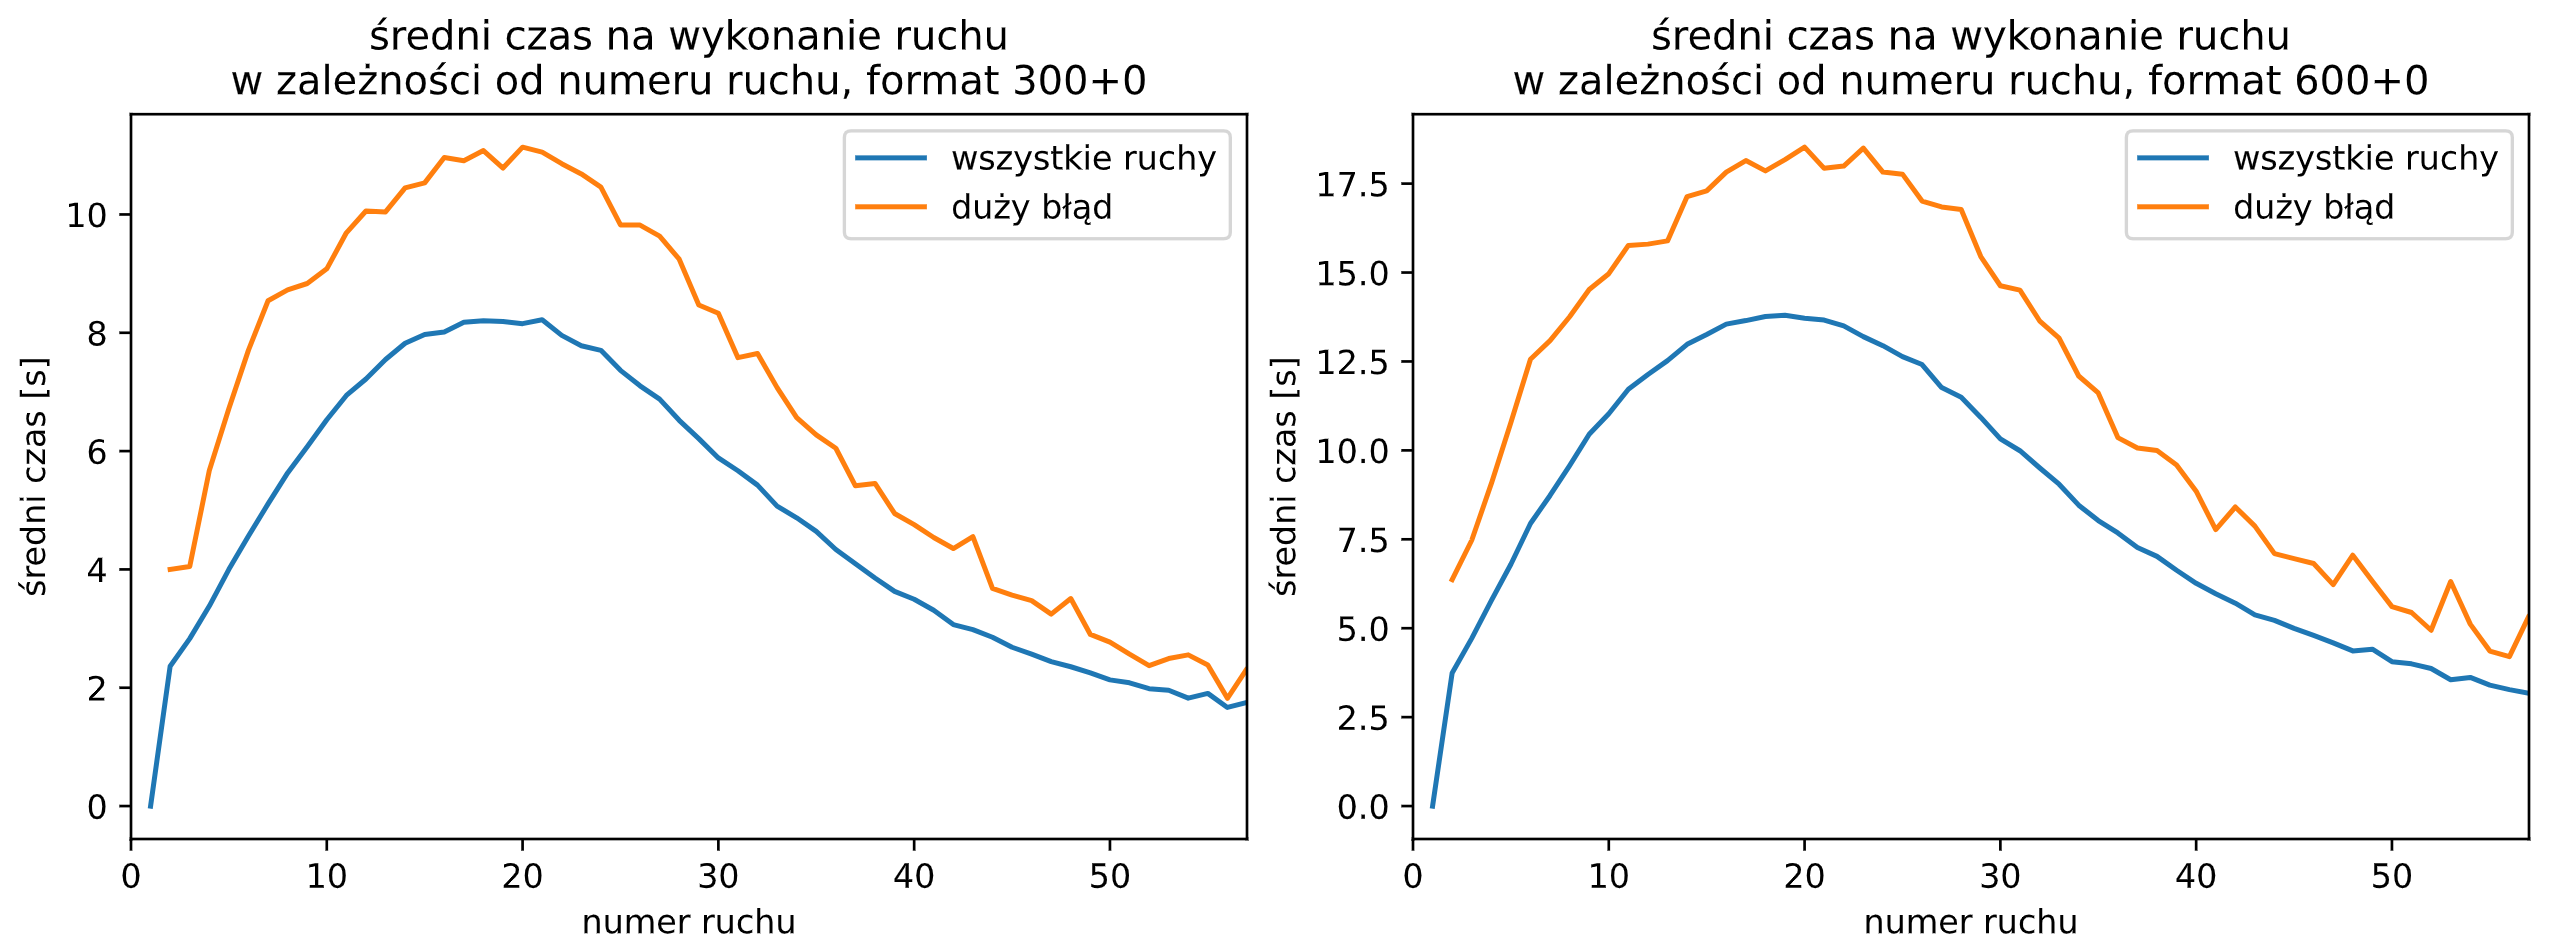
\includegraphics[width=11cm]{../Formatka/sr_czas_na_ruch.png}
		\caption{Średni czas na wykonanie ruchu dla analizowanych formatów czasowych wraz z zaznaczonym rozstępem międzykwartylowym. Osobno wszystkie ruchy i ruchy oznaczone przez silnik jako błąd.}
		\label{rys:sr_czas_na_ruch}
	\end{figure}
\end{frame}

\begin{frame}{Zależność między indeksem ruchu, a poświęconym czasem}
	Po oznaczeniu:\\ 
	\textit{D} jako zmienną określającą skomplikowanie pozycji,\\ \textit{T} - zmienną określającą czas na wykonanie ruchu w danej pozycji,\\ \textit{B} - zdarzenie polegające na tym, że posunięcie jest błędne\\
	 i przy założeniu, że \textit{T} jest silnie dodatnio skorelowane z \textit{D}, według prawdopodobieństwa otrzymujemy:
	\begin{equation*}
		P(B|D>d_0) > P(B|D\leq d_0) \rightarrow P(B|T>t_0) > P(B|T\leq t_0)
	\end{equation*}
	gdzie $d_0$ i $t_0$ określają punkty, od których według wybranej miary można określić, że pozycja jest skomplikowana ($D>d_0$) i czas na wykonanie posunięcia jest długi ($T>t_0$).
	
	
	Może to tłumaczyć wyższą średnią czasu na wykonanie błędnego posunięcia w porównaniu do zbioru wszystkich posunięć.
\end{frame}

\begin{frame}{Zależność między indeksem ruchu, a poświęconym czasem}
\begin{figure}[H]
	\centering
	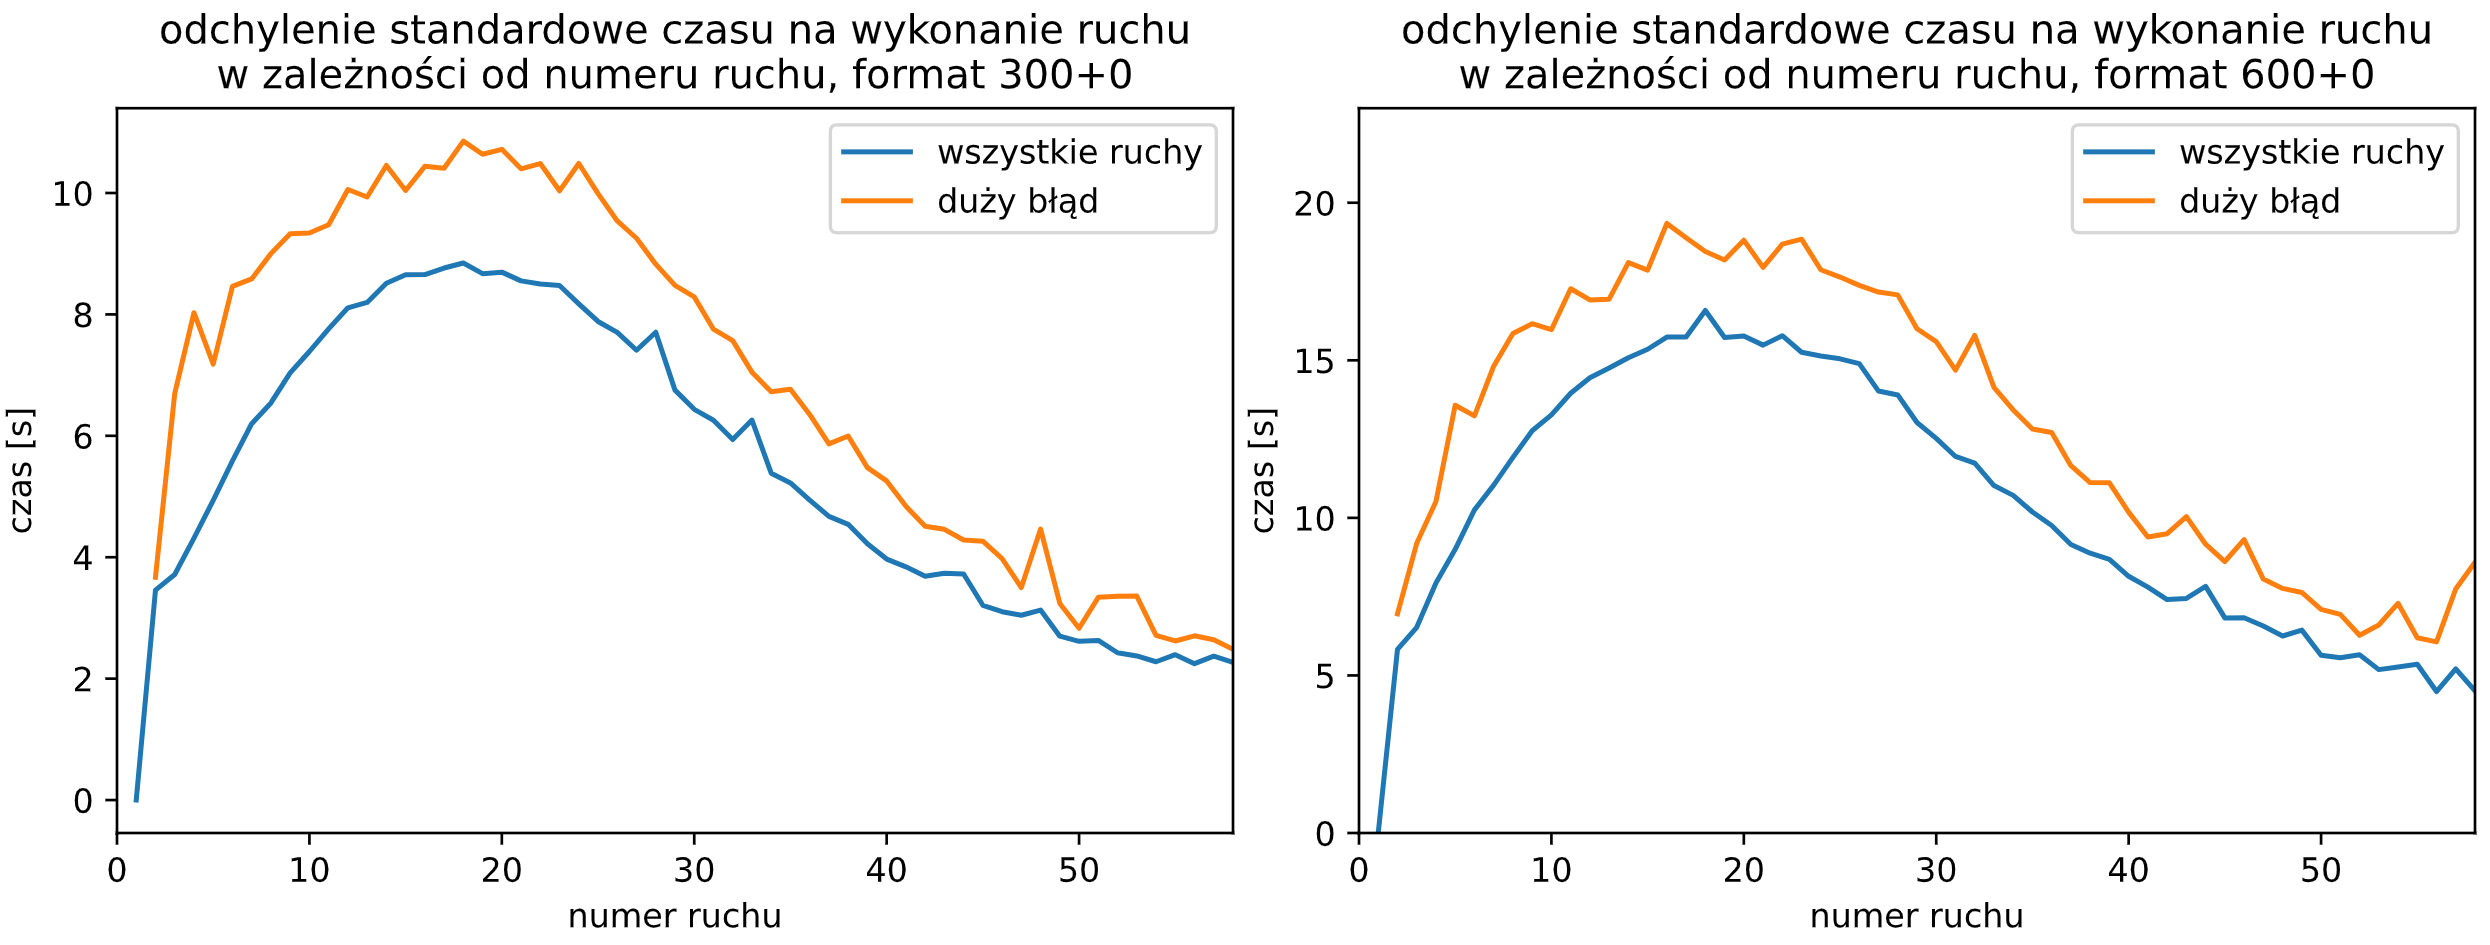
\includegraphics[width=11cm]{../Formatka/std_czas_na_ruch.png}
	\caption{Odchylenie standardowe czasu na wykonanie ruchu dla analizowanych formatów czasowych. Osobno wszystkie ruchy i ruchy oznaczone przez silnik jako błąd.}
	\label{rys:std_czas_na_ruch}
\end{figure}
\end{frame}
\begin{frame}{Zależność między indeksem ruchu, a poświęconym czasem}
	\begin{figure}[H]
		\centering
		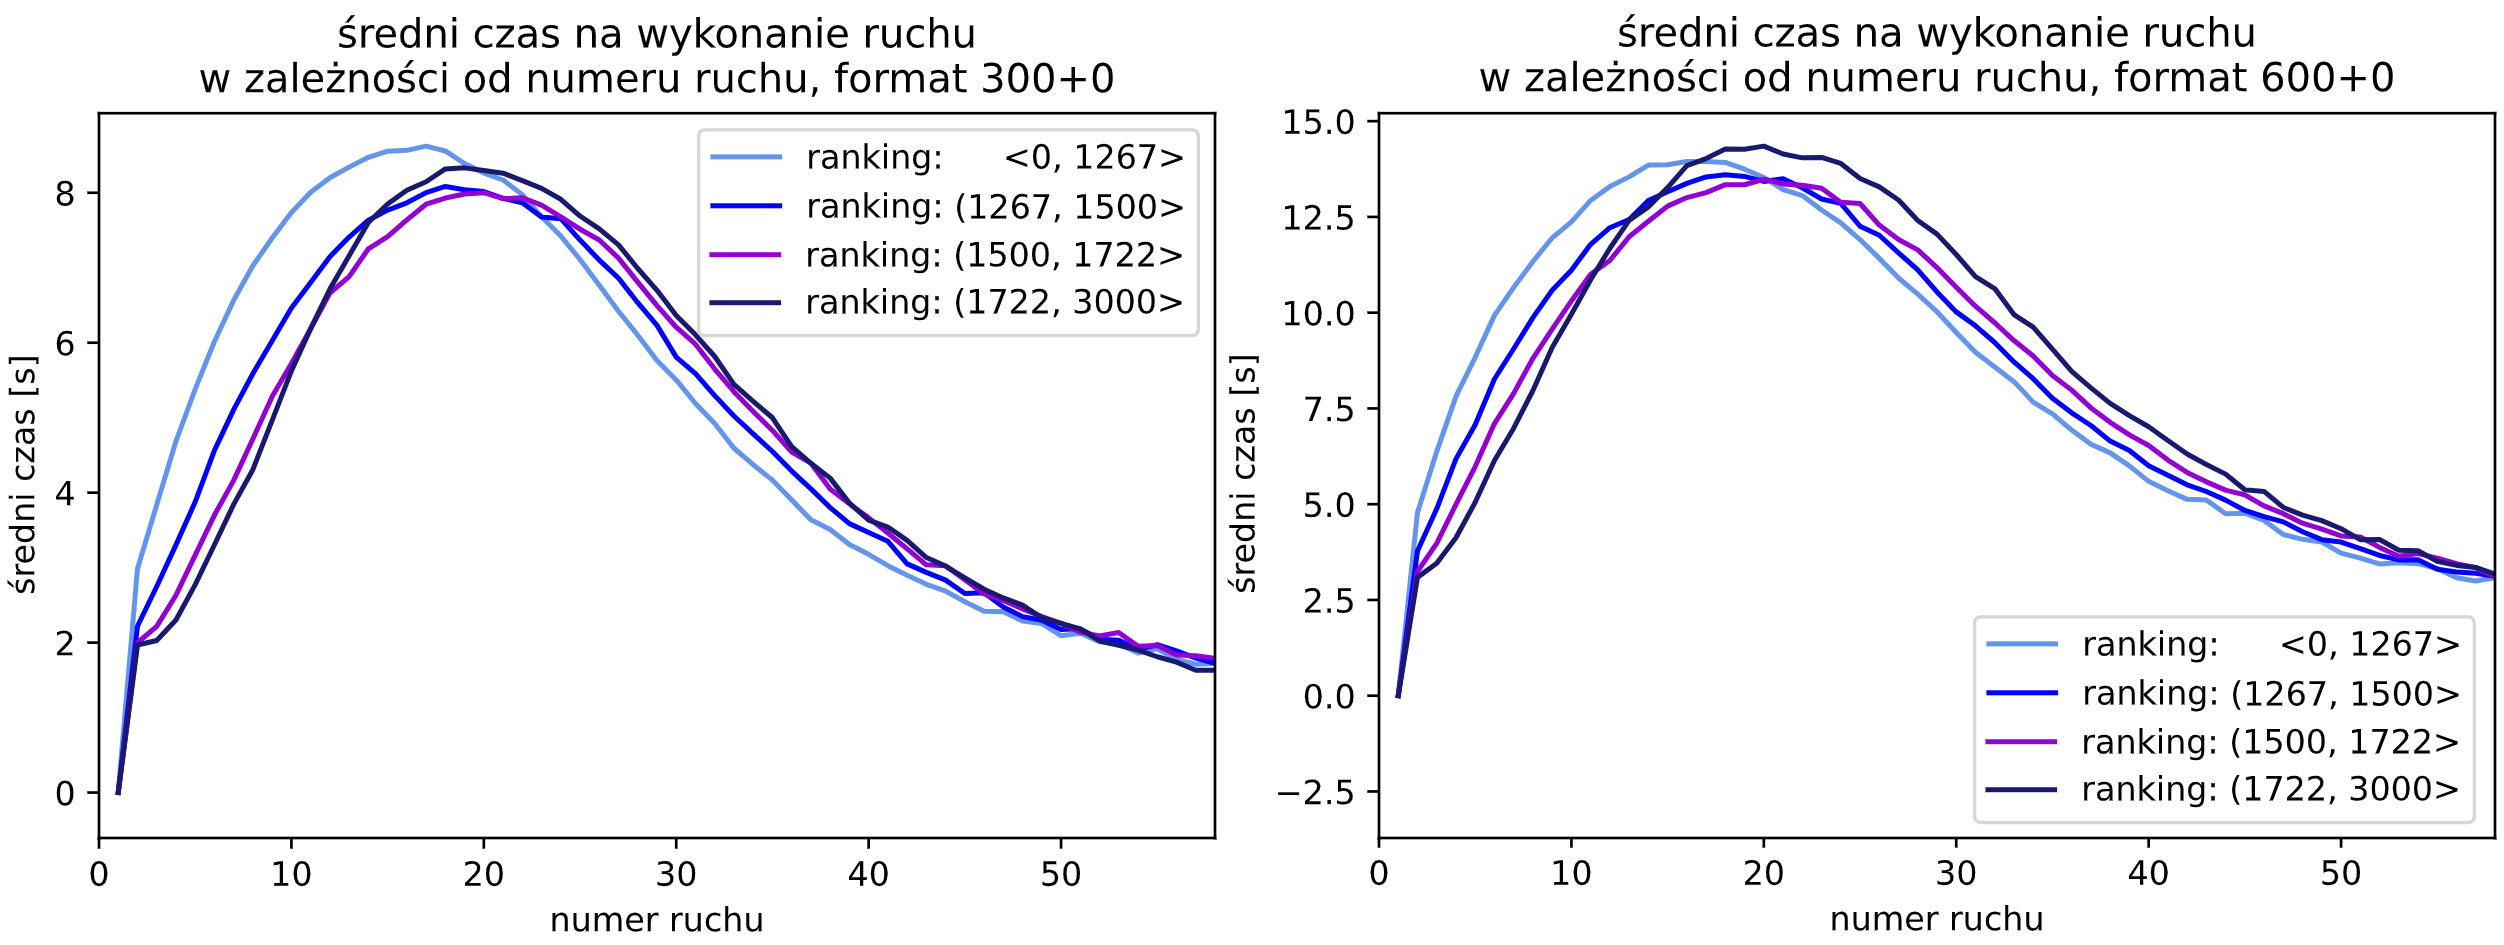
\includegraphics[width=11cm]{../Formatka/sr_czas_na_ruch_ELO_1.png}
		\caption{Średni czas na wykonanie ruchu dla dla graczy z różnych przedziałów rankingowych. Wszystkie posunięcia.}
		\label{rys:sr_czas_na_ruch_ELO_1}
	\end{figure}
\end{frame}

\begin{frame}{Zależność między indeksem ruchu, a poświęconym czasem}
	\begin{figure}[H]
		\centering
		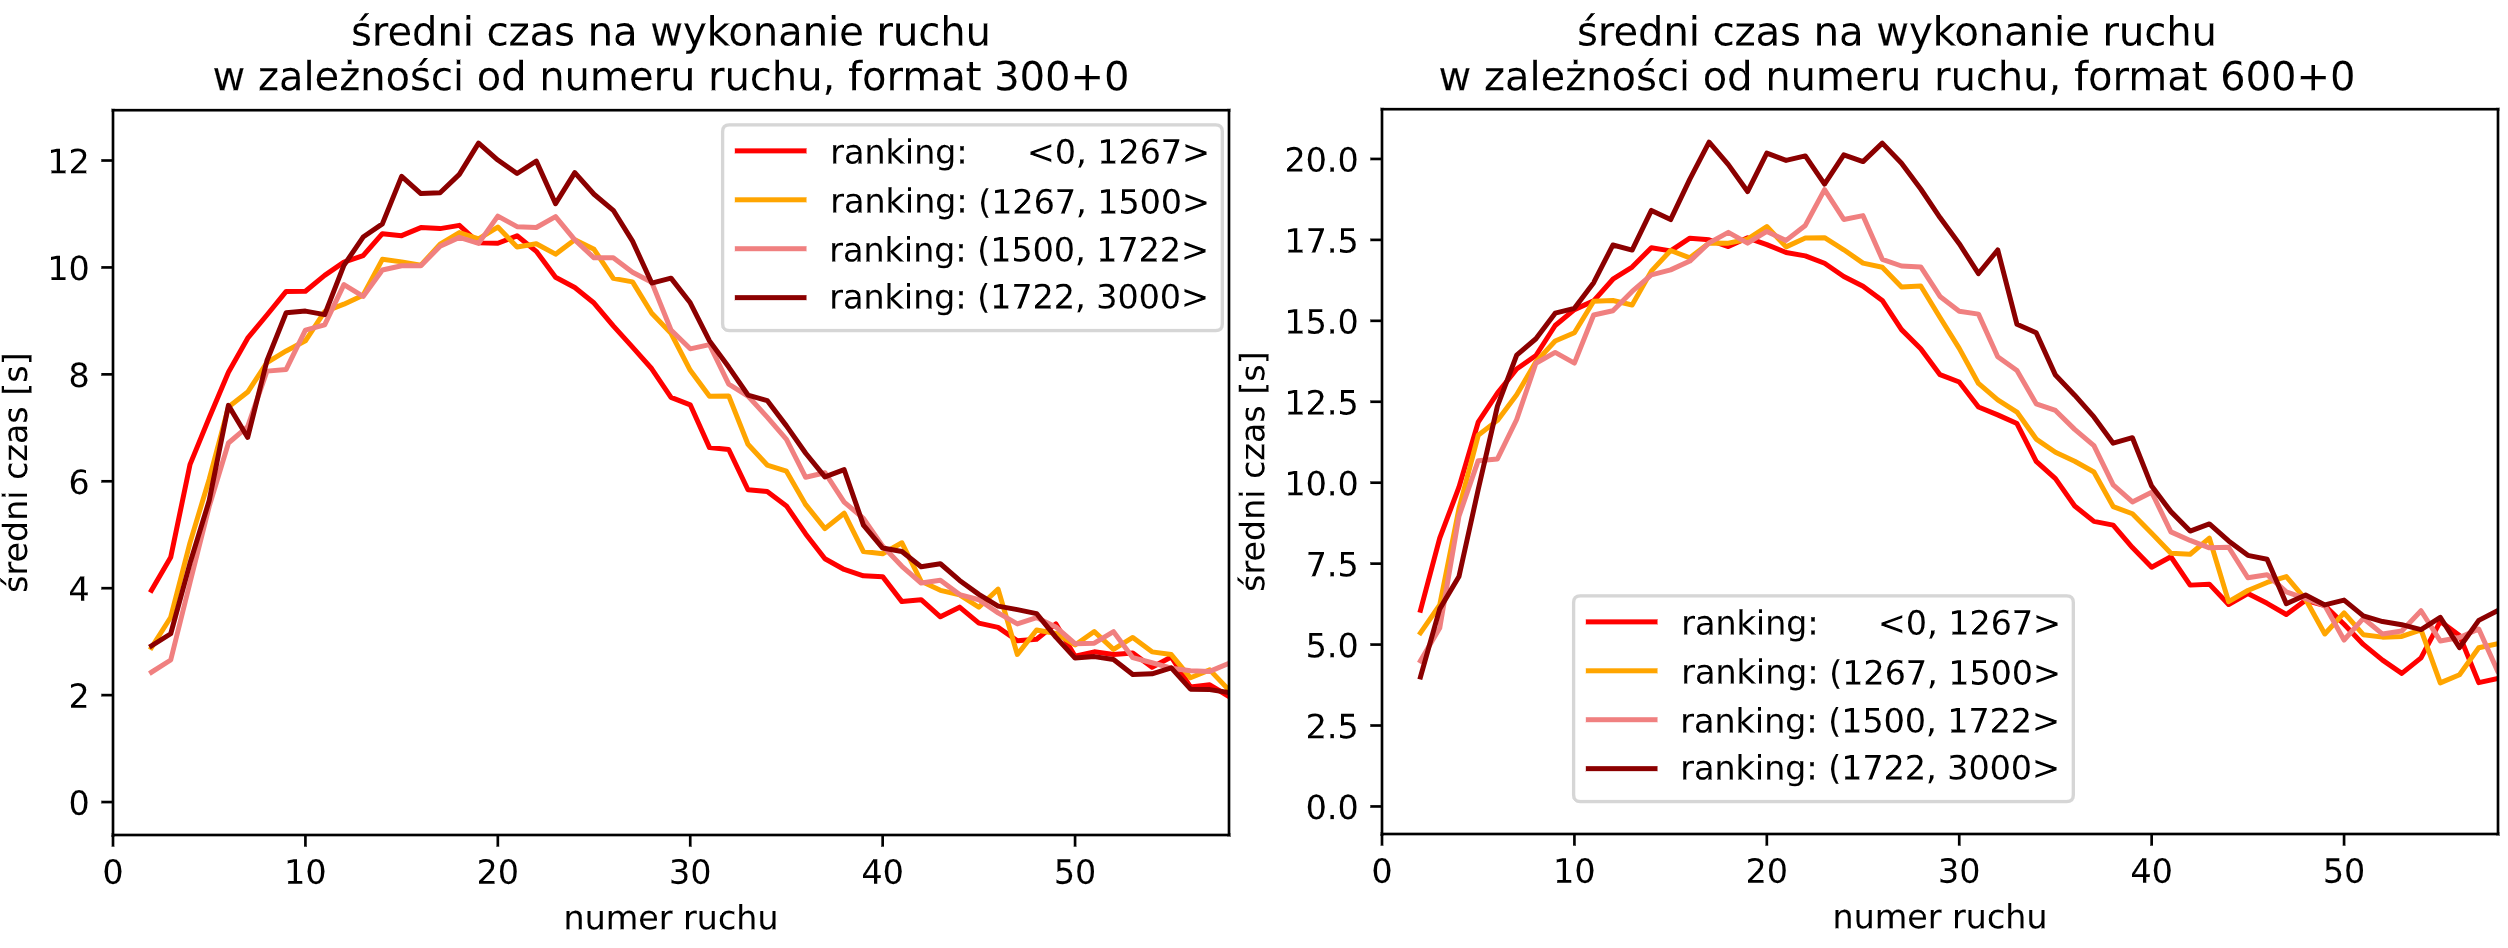
\includegraphics[width=11cm]{../Formatka/sr_czas_na_ruch_ELO_2.png}
		\caption{Średni czas na wykonanie ruchu dla dla graczy z różnych przedziałów rankingowych. Posunięcia oznaczone przez silnik jako błąd.}
		\label{rys:sr_czas_na_ruch_ELO_2}
	\end{figure}
\end{frame}

\begin{frame}{Zależność między indeksem ruchu, a poświęconym czasem}
\begin{figure}[H]
	\centering
	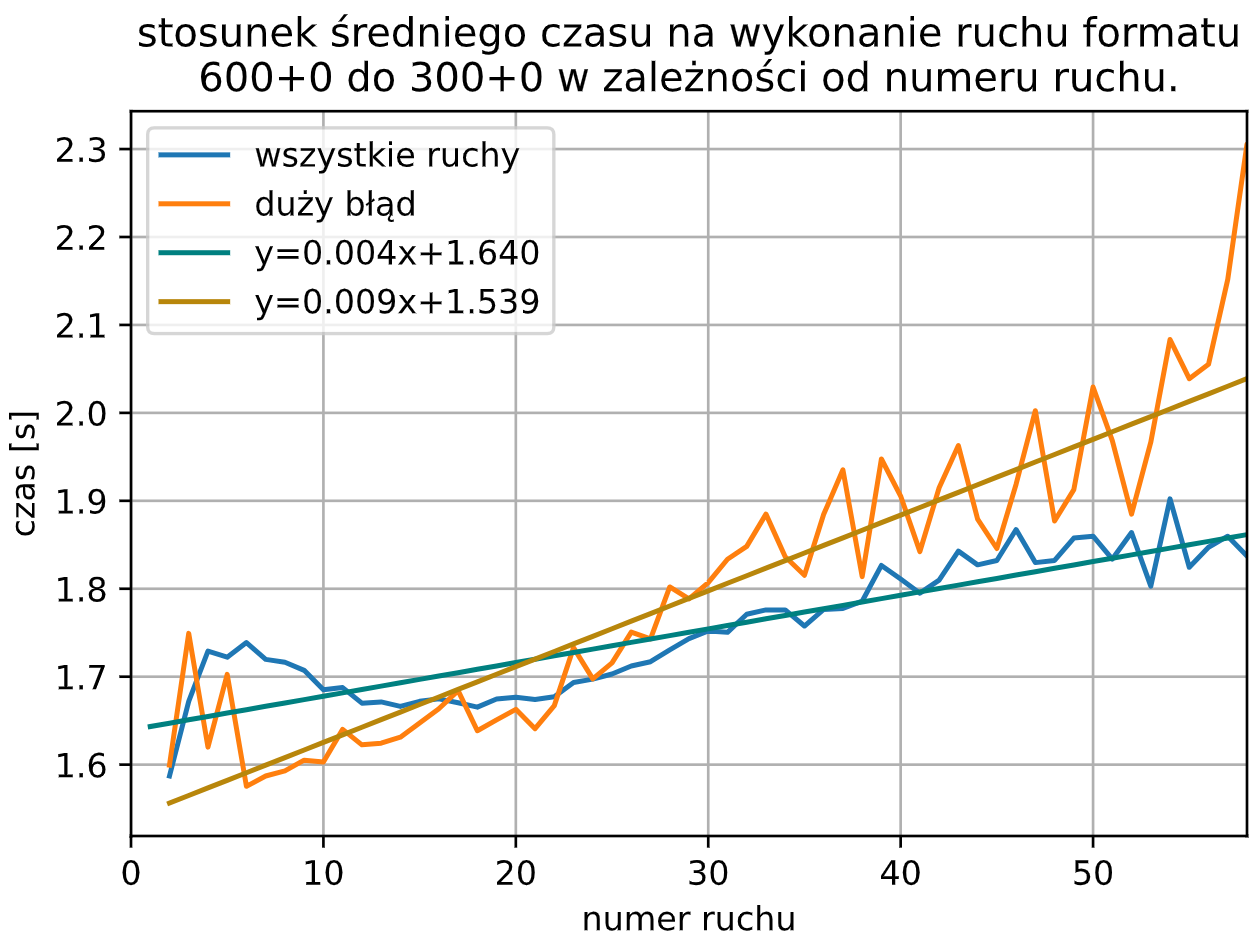
\includegraphics[width=7cm]{../Formatka/stosunek_sr_czas.png}
	\caption{Stosunek średniego czasu na wykonanie ruchu w formacie 600+0 do czasu w formacie 300+0. Zaznaczone proste regresji obrazujące trend.}
	\label{rys:stosunek_sr_czas}
\end{figure}
\end{frame}


\begin{frame}{Zależność między indeksem ruchu, a poświęconym czasem}
	\begin{figure}[H]
		\centering
		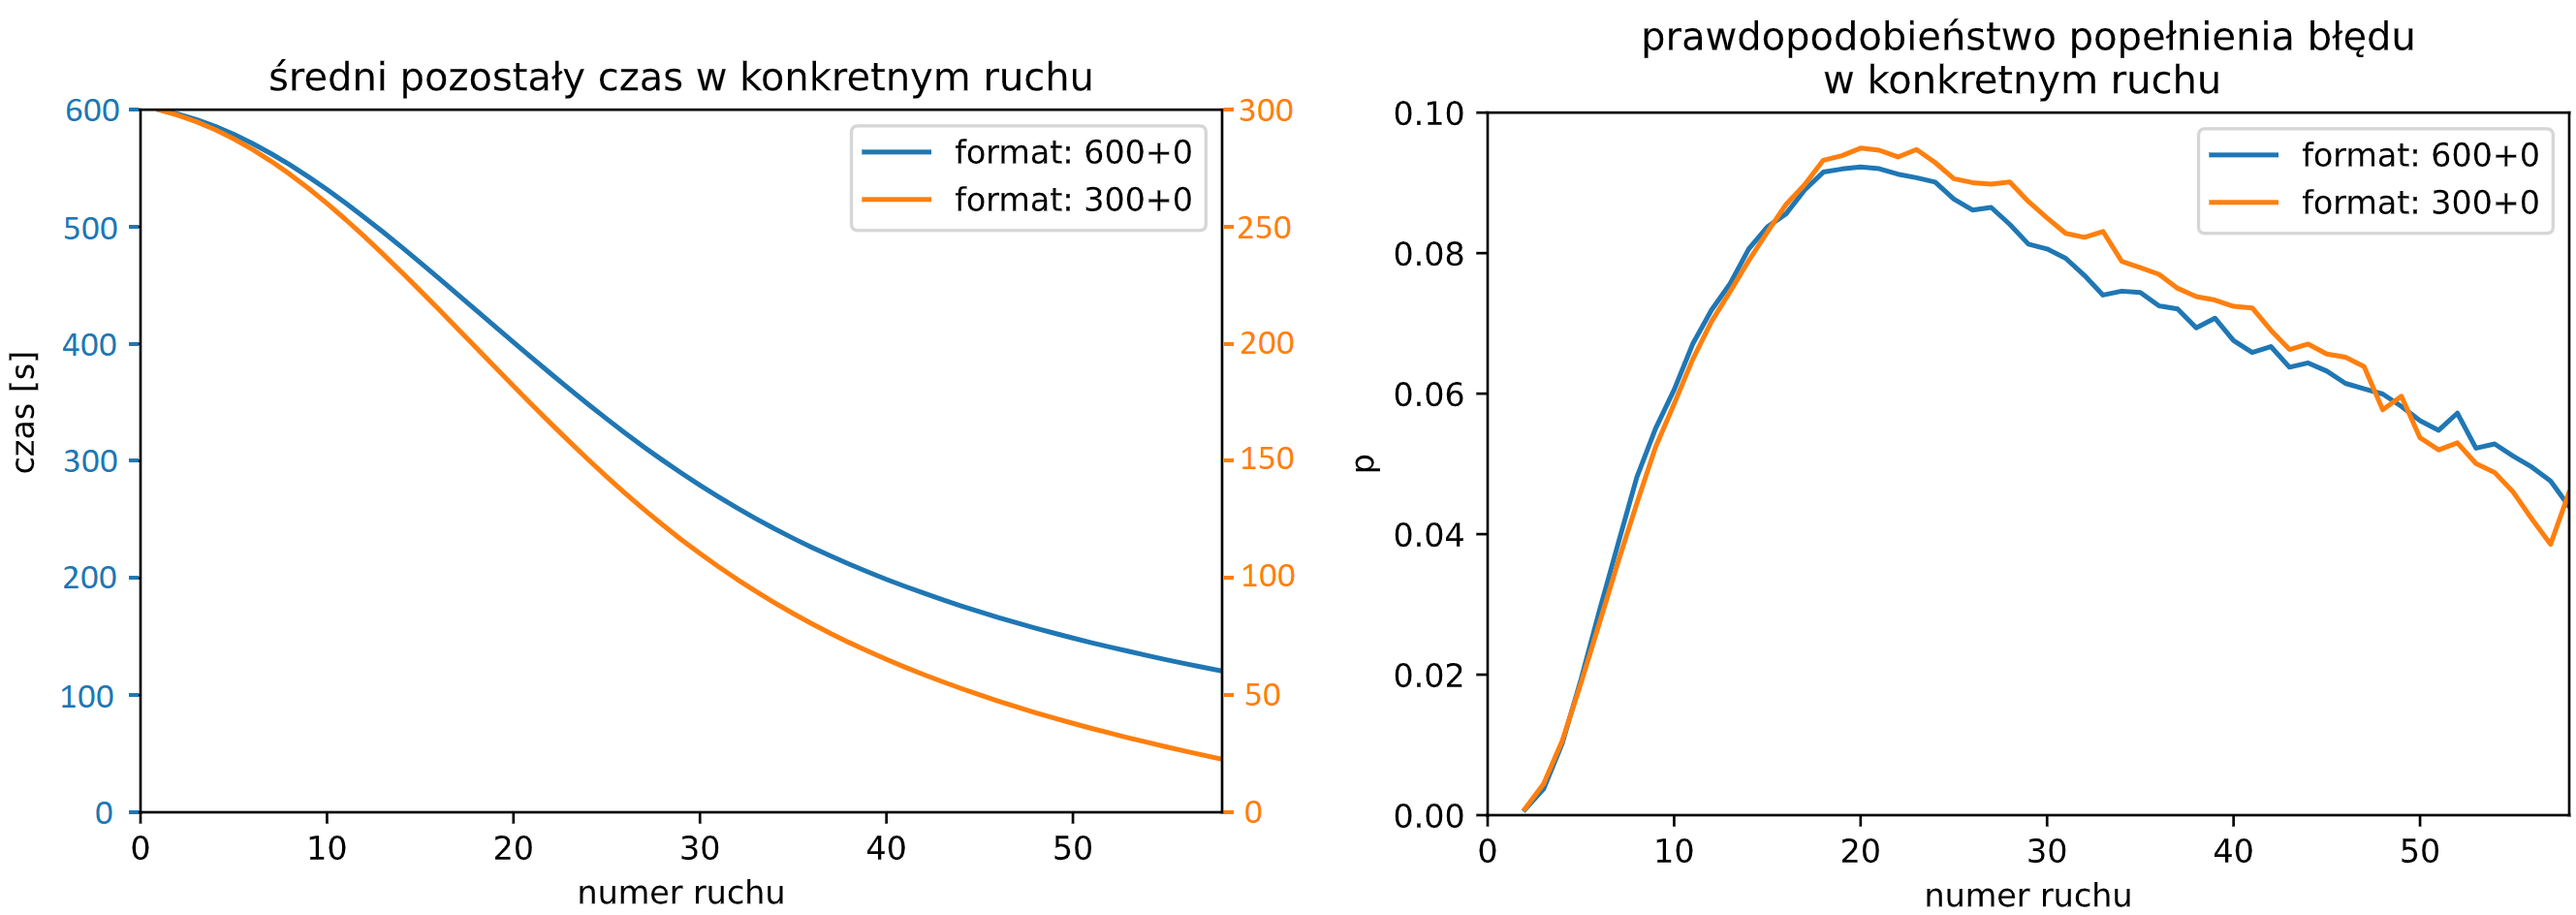
\includegraphics[width=11cm]{../Formatka/pozostaly_czas.png}
		\caption{
			Pierwszy wykres -- zestawienie średniego pozostałego czasu w formatach 600+0 oraz 300+0. W celu lepszego porównania zastosowane osobne osie dla każdego formatu. Drugi wykres -- empiryczne prawdopodobieństwo popełnienia błędu w konkretnym ruchu.}
		\label{rys:pozostaly_czas}
	\end{figure}
\end{frame}

\begin{frame}{Zależność między indeksem ruchu, a poświęconym czasem}
\begin{figure}[H]
	\centering
	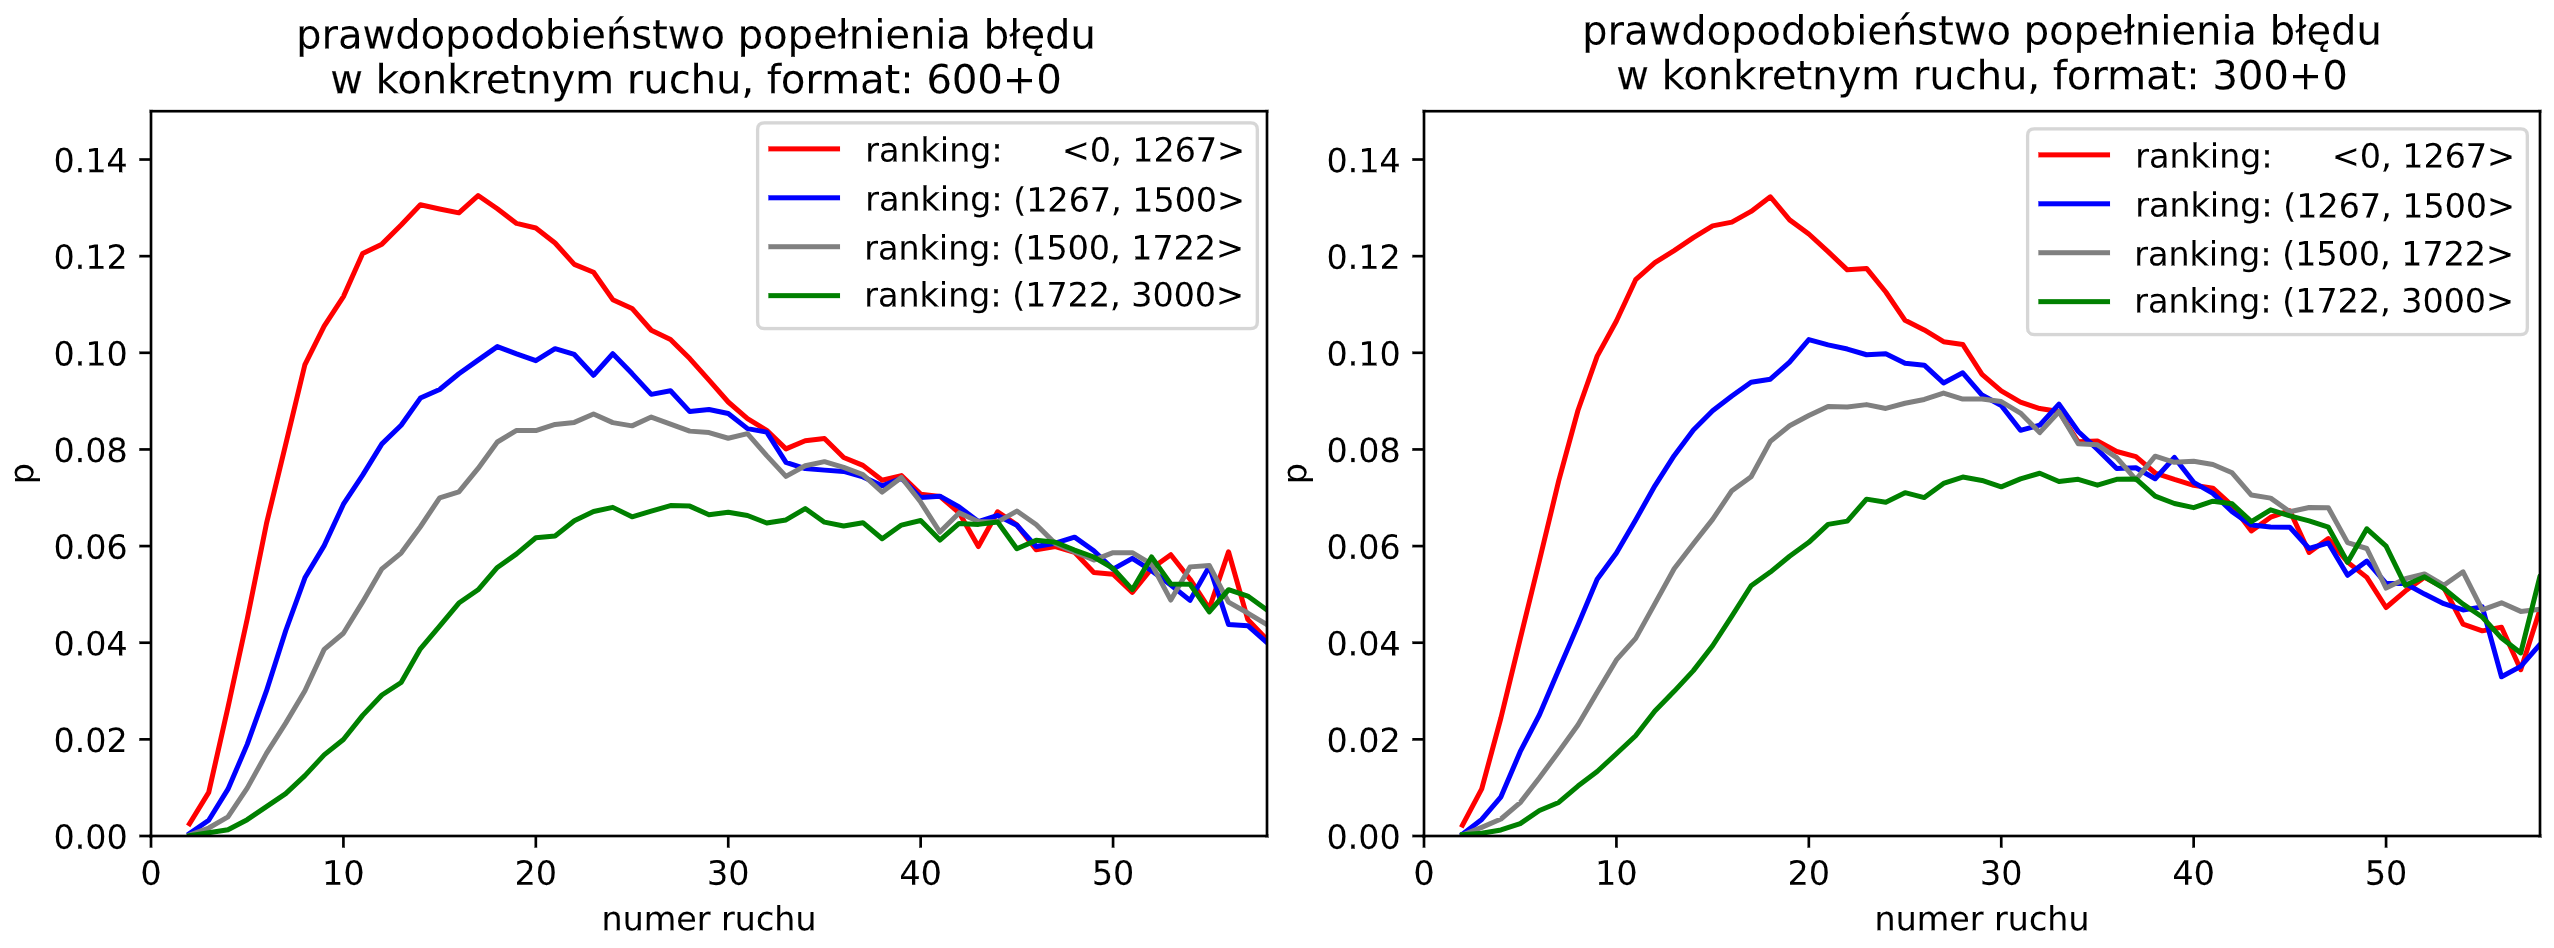
\includegraphics[width=11cm]{../Formatka/prawd_blad_ELO.png}
	\caption{Prawdopodobieństwo popełnienia błędu w konkretnym ruchu dla różnych przedziałów rankingowych.}
	\label{rys:prawd_blad_ELO}
\end{figure}
\end{frame}

\begin{frame}{Zależność między indeksem ruchu, a poświęconym czasem}
	\begin{equation*}
		X_i =
		\begin{cases}
			1, & \text{gdy w $i$-tym ruchu został popełniony błąd}\\
			0, & \text{gdy w $i$-tym ruchu nie został popełniony błąd}
		\end{cases}       
	\end{equation*}
\begin{multline*}
	\begin{split}
		& P(X_1 = 1 \vee X_2 = 1 \vee \dots \vee X_n = 1) =\\
		& = 1 - P(X_1 = 0, X_2 = 0,\dots, X_n = 0) = \\
		& = P(X_1 = 0)P(X_2 = 0)\dots P(X_n = 0) = \\
		& = \prod_{i=1}^{n}P(X_i=0)
	\end{split}
\end{multline*}
\end{frame}

\begin{frame}{Zależność między indeksem ruchu, a poświęconym czasem}
	\scriptsize
	\begin{table}[H]
		\caption{Szansa na popełnienie błędu w pierwszych \textit{n} ruchach dla gracza z określonego przedziału rankingowego z rozdzieleniem na formaty ,,600+0'' i ,,300+0''}
		\centering
		\begin{tabular}{|l|r|r|r|r|r|r|l}
			\cline{1-7}
			\textbf{\begin{tabular}[c]{@{}l@{}}\textit{n} pierwszych \\ ruchów\end{tabular}} & \multicolumn{2}{l|}{\textbf{n = 10}}                                      & \multicolumn{2}{l|}{\textbf{n = 20}}                                      & \multicolumn{2}{l|}{\textbf{n = 30}}                                      & \textbf{} \\ \cline{1-7}
			\textbf{centyl\hphantom{ } \textbackslash \hphantom{ } format}                                   & \multicolumn{1}{l|}{\textbf{600+0}} & \multicolumn{1}{l|}{\textbf{300+0}} & \multicolumn{1}{l|}{\textbf{600+0}} & \multicolumn{1}{l|}{\textbf{300+0}} & \multicolumn{1}{l|}{\textbf{600+0}} & \multicolumn{1}{l|}{\textbf{300+0}} &           \\ \cline{1-7}
			\textbf{0-25\%}                                                         & 43,36\%                             & 40,72\%                             & 85,50\%                             & 84,33\%                             & 95,32\%                             & 94,96\%                             &           \\ \cline{1-7}
			\textbf{25\%-50\%}                                                      & 25,52\%                             & 22,09\%                             & 71,56\%                             & 68,63\%                             & 89,38\%                             & 88,66\%                             &           \\ \cline{1-7}
			\textbf{50\%-75\%}                                                      & 15,58\%                             & 12,42\%                             & 58,86\%                             & 56,27\%                             & 83,08\%                             & 82,93\%                             &           \\ \cline{1-7}
			\textbf{75\%-100\%}                                                     & 6,76\%                              & 5,63\%                              & 40,78\%                             & 38,66\%                             & 70,27\%                             & 70,40\%                             &           \\ \cline{1-7}
		\end{tabular}
		\label{tab:blad_w_n_ruchach} 
	\end{table}
\normalsize
\end{frame}

\begin{frame}{Zależność między czasem poświęconym na ruch, a jego oceną}
\begin{figure}[H]
	\centering
	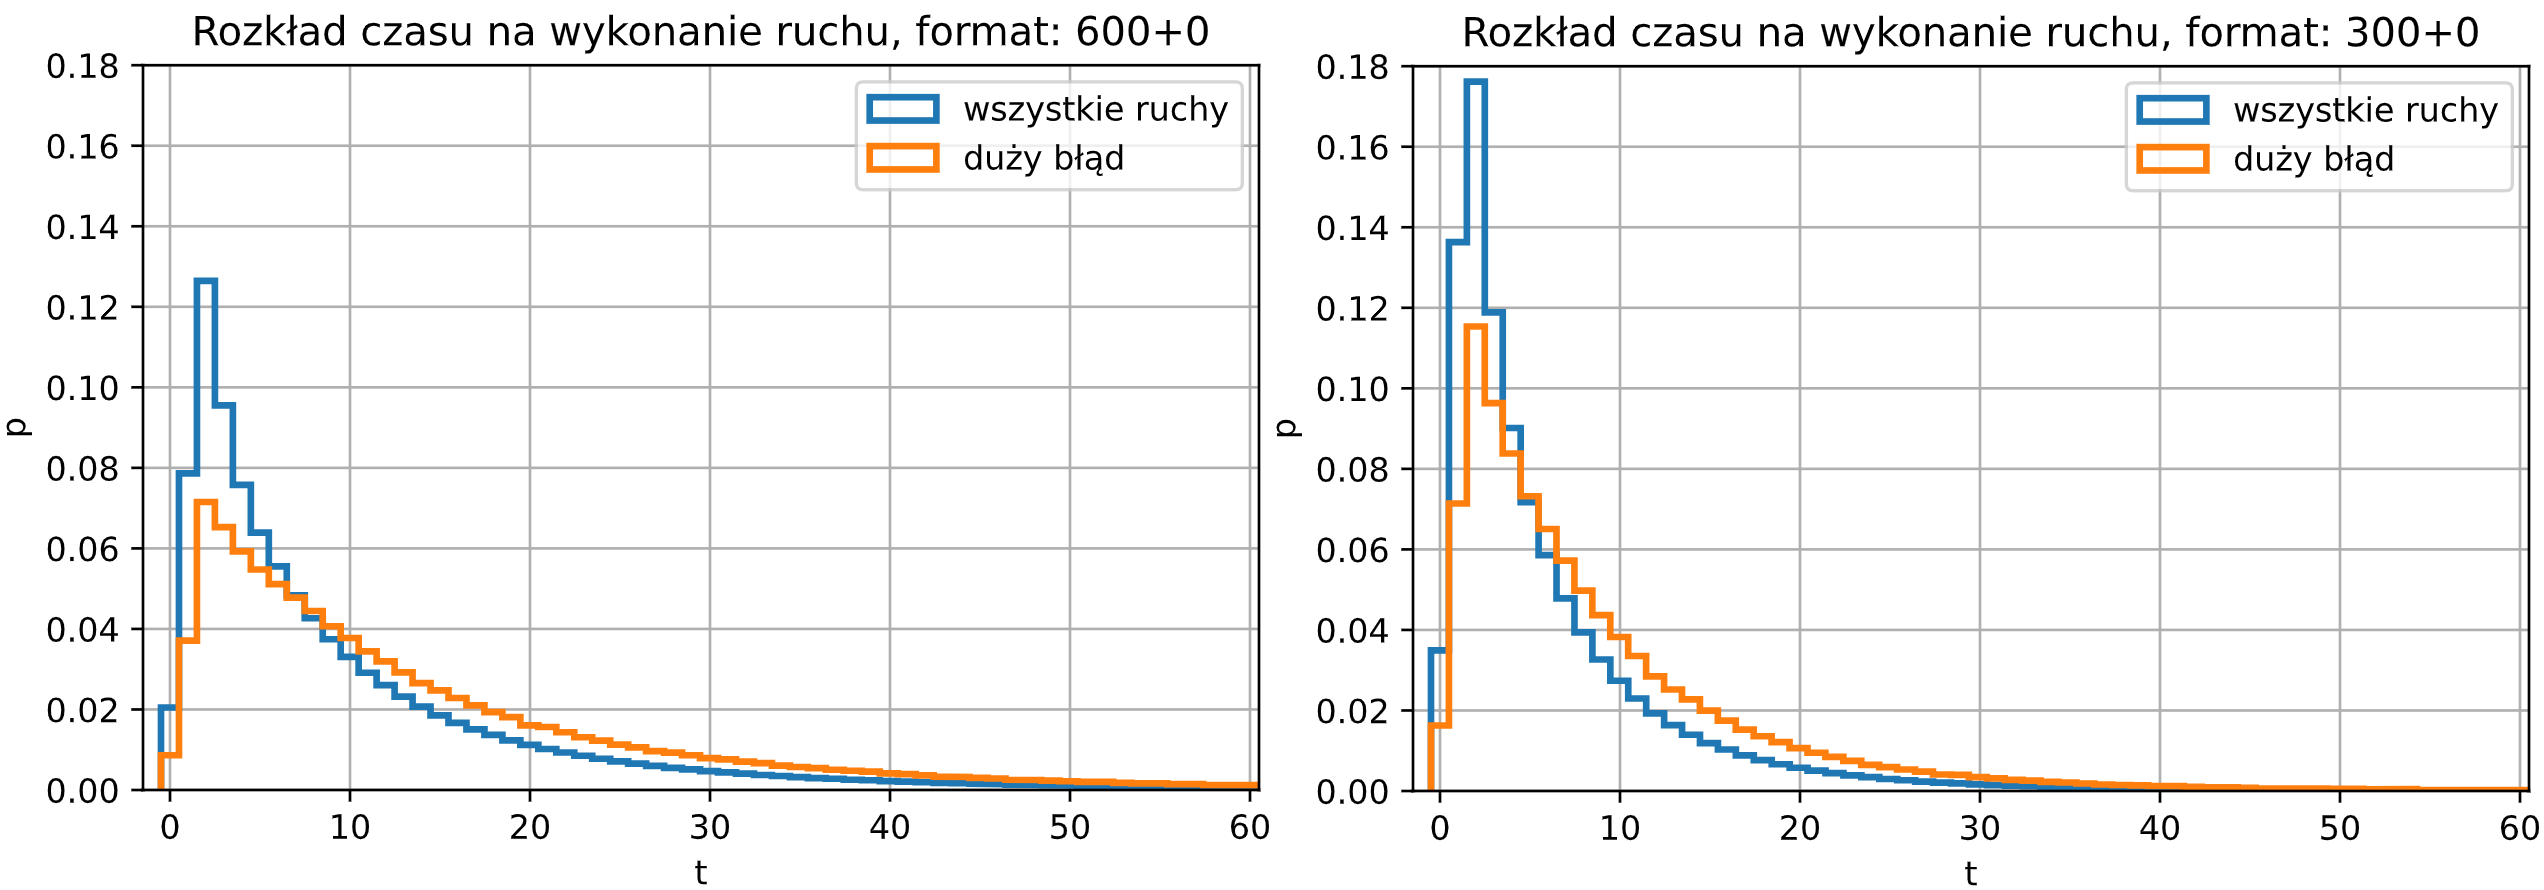
\includegraphics[width=11cm]{../Formatka/rozklad_czasu.png}
	\caption{Rozkład czasu poświęconego na wykonanie posunięcia dla formatów ,,600+0'' i ,,300+0''. Osobno wszystkie posunięcia i posunięcia błędne}
	\label{rys:rozklad_czasu}
\end{figure}
\end{frame}

\begin{frame}{Zależność między czasem poświęconym na ruch, a jego oceną}
	\begin{figure}[H]
		\centering
		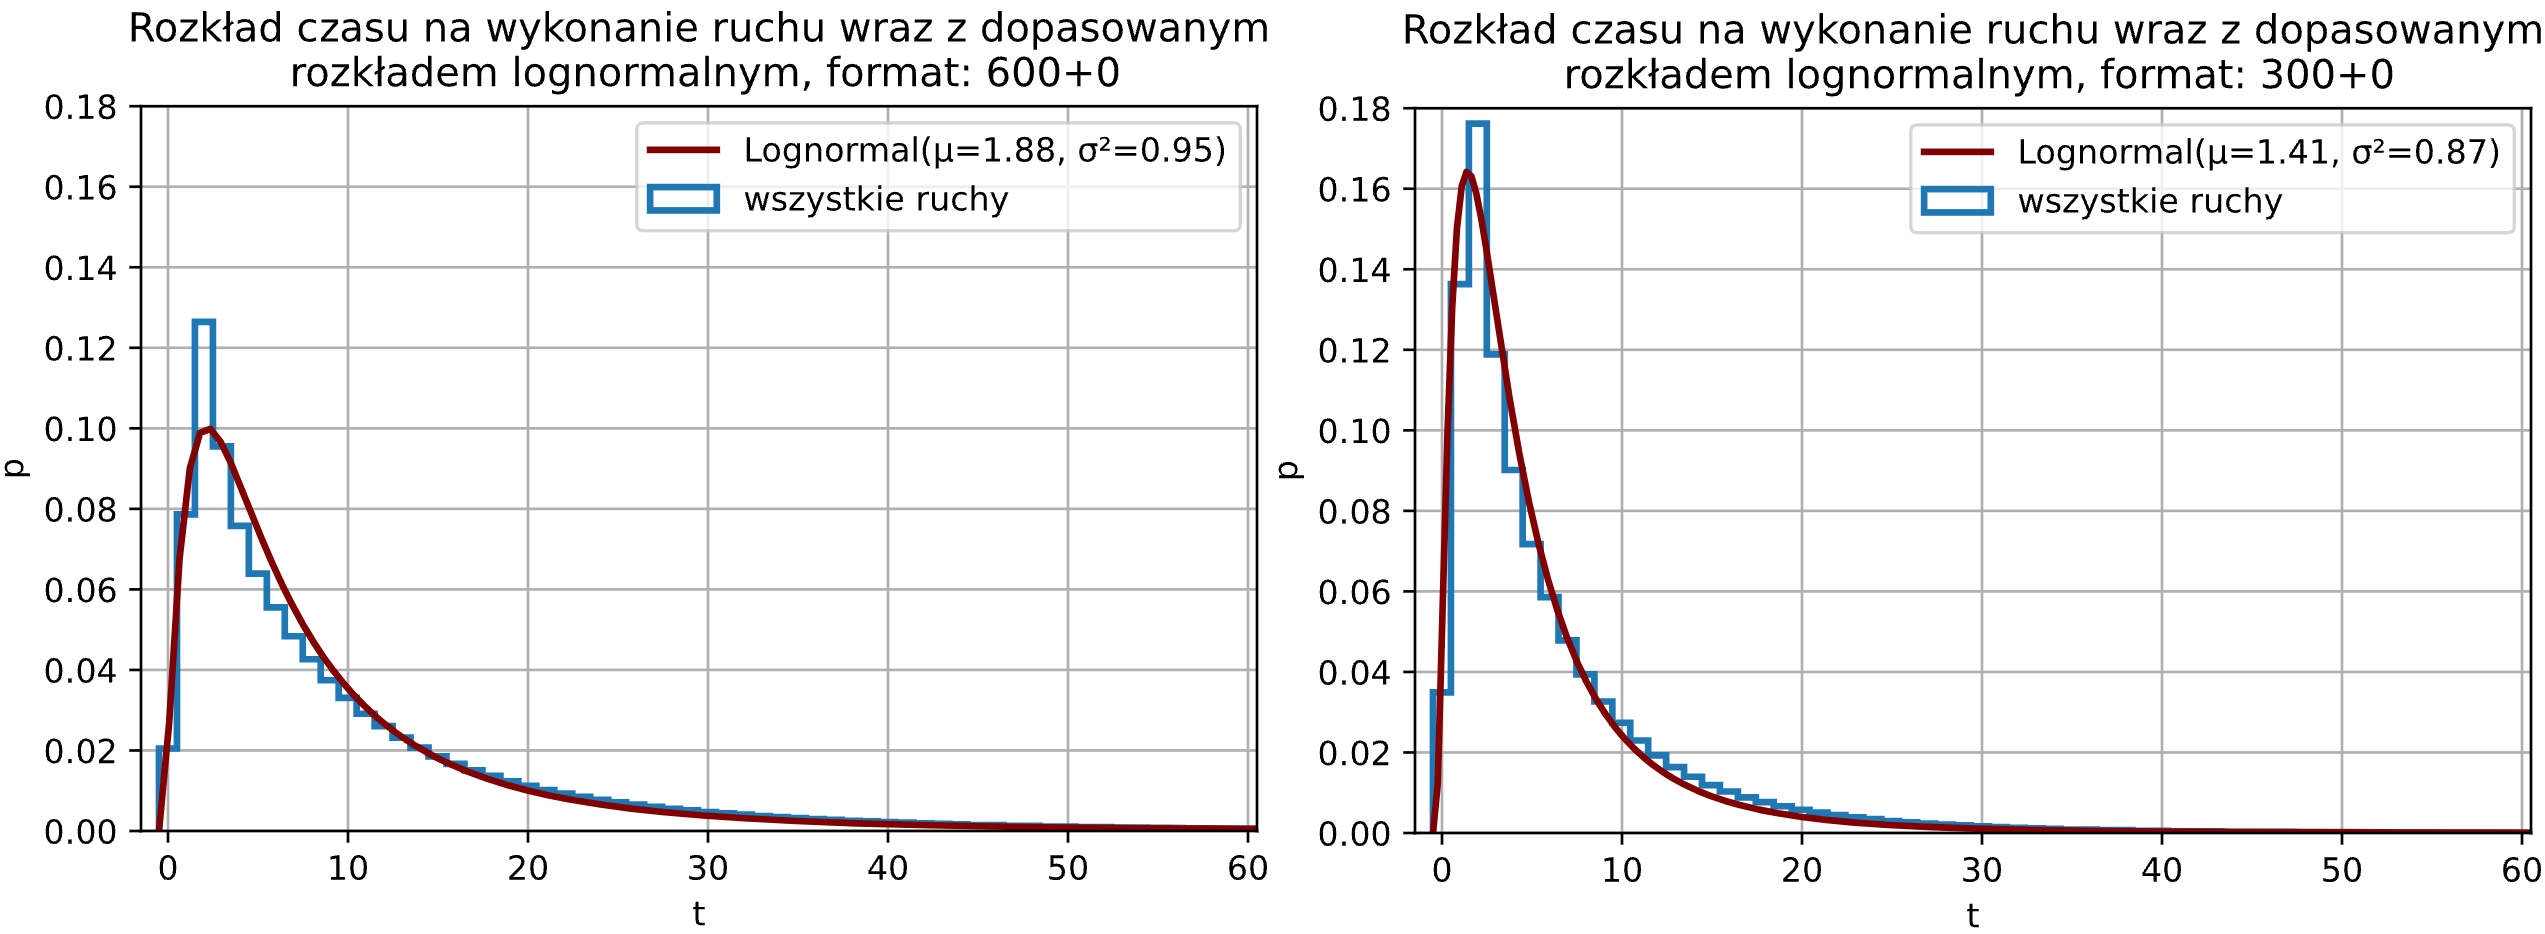
\includegraphics[width=11cm]{../Formatka/rozklad_lognorm.png}
		\caption{Rozkład czasu poświęconego na wykonanie posunięcia dla formatów ,,600+0'' i ,,300+0'' z dopasowanym rozkładem log-normalnym.}
		\label{rys:rozklad_lognorm}
	\end{figure}
\end{frame}
\begin{frame}{Zależność między czasem poświęconym na ruch, a jego oceną}
	\begin{figure}[H]
		\centering
		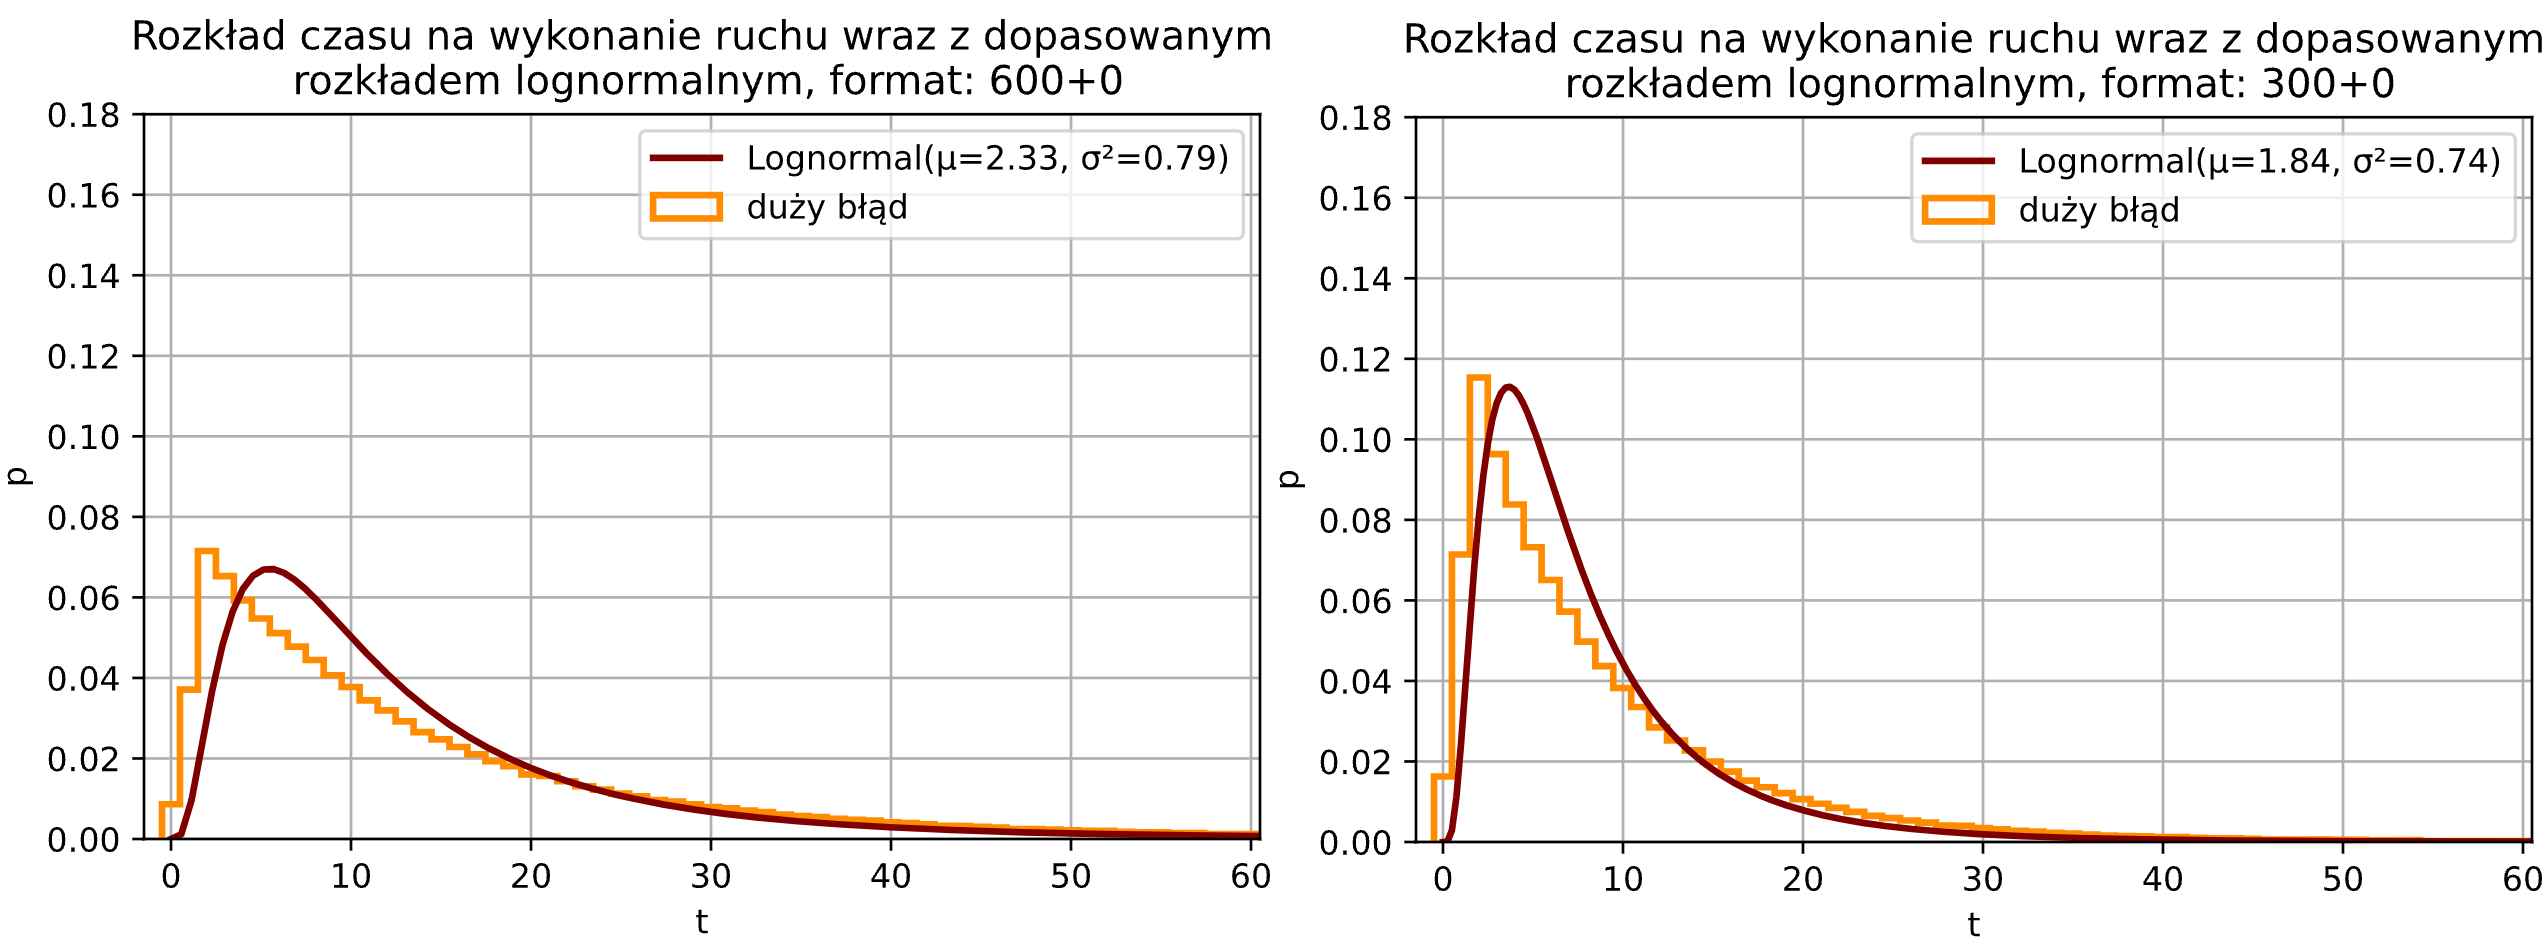
\includegraphics[width=11cm]{../Formatka/rozklad_lognorm2.png}
		\caption{Rozkład czasu poświęconego na wykonanie posunięcia dla formatów ,,600+0'' i ,,300+0'' z dopasowanym rozkładem log-normalnym. Zestaw ruchów błędnych.}
		\label{rys:rozklad_lognorm2}
	\end{figure}
\end{frame}

\section{Podsumowanie}

\begin{frame}{Wnioski}
	\begin{itemize}
		\item 95\% gier kończy się w 57 ruchach
		\item błędne posunięcie zajmuje średnio dłużej niż standardowe 
		\begin{itemize}
			\item dla każdego rankingu i numeru ruchu
			\item błędne posunięcie ma też zawsze większą wariancje
		\end{itemize}
		\item największa szansa na błąd umiejscowiona jest w okolicach 20 ruchu
		\item gracze z wyższym rankingiem szybciej wykonują ruchy początkowe, dłużej te z największą szansą na błąd
		\begin{itemize}
			\item w odniesieniu do graczy z niższym rankingiem
			\item więcej czasu poświęconego na posunięcie\\ w okolicy 20 ruchu $\rightarrow$ mniejsza szansa na błąd
		\end{itemize}
		
		
	\end{itemize}
\end{frame}

\begin{frame}{Wnioski}
	\begin{itemize}
		\item największa szansa na błąd
		\begin{itemize}
			\item słabsi gracze -- dużo więcej błędów na początku (ruchy 1 -- 20)
			\item słabsi gracze -- więcej błędów w środkowej części gry (ruchy 20 -- 30)
			\item słabsi gracze -- podobna liczba błędów w fazie końcowej (ruchy 30+)
		\end{itemize} 
		\item lepsi gracze DŁUŻEJ wykonują ruchy BŁĘDNE
		\item różnice między formatami
		\begin{itemize}
			\item dla ,,600+0'' ruchy zajmują nieliniowo więcej czasu, niż dla ,,300+0'' 
			\item dla ,,300+0'' gracze są zmuszeni szybko wykonywać ruchy późniejsze.
		\end{itemize} 
\end{itemize}
\end{frame}

\begin{frame}{Wnioski}
	\begin{itemize}
		\item 10 pierwszych ruchów (otwarcie), 
		\begin{itemize}
			\item istotna różnica w popełnieniu przynajmniej jednego  błędu między rankingami
			\item przykładowo: format ,,300+0''\\ 
			\phantom{4}5,63\% szansy na błąd dla graczy powyżej centylu 75, \\
			40,72\% szansy na błąd dla graczy poniżej centylu 75, \\
		\end{itemize}	
	\end{itemize}
\end{frame}


\begin{frame}{Dalsza praca}
	\begin{itemize}
		\item stworzenie odpowiedniej miary i wzięcie pod uwagę poziomu skomplikowania pozycji
		\begin{itemize}
			\item potrzebna dużo większa moc obliczeniowa	
		\end{itemize}
	
		\item stworzenie odpowiedniej miary do określania błędów (innej niż Stockfish)
		\begin{itemize}
			\item sprawdzenie zgodności wyników
			\item potrzebna dużo większa moc obliczeniowa	
		\end{itemize}
	\end{itemize}
	
\end{frame}

\begin{frame}{Bibliografia}
	\bibliography{bibliografia} 
\end{frame}

\begin{frame}{Pytania?}
	%całość pracy dostępna pod adresem:\\ \url{https://github.com/rogulforce/Chess}
\end{frame}

\end{document}
